\section{Ex2.12 Data-set}\label{sec:Data_set}

\subsection{Testo esercizio}
Il file \textit{velocityy.dat} contiene un elenco di valori cosi disposti:\\

\begin{tabular}{cc}
    $t0$&$v0$\\
    $t1$&$v1$\\
    $..$&$..$\\
    $tn$&$vn$\\
\end{tabular}\\

corrispondenti al tempo $t(i)$, misurato in secondi, e alla velocità $v(i)$, 
misurata in metri al secondo, per la traiettoria di un proiettile.

\begin{itemize}
    \item[a)] Leggere il file di dati, e popolare le matrici $t$ e $v$.
    
    \item[b)] Graficare $v$ in funzione di $t$.
 
    \item[c)] Tracciare le posizioni $(x, y)$ dell'oggetto in un plot con $x$ e 
    $y$ sui due grafici, uno sopra l'altro.
\end{itemize}   

\subsection{Svolgimento}
L'esercizio \'e stato semplice. Inizialmente avevo inserito $\rho=7500$ 
direttamente dentro la funzione, successivamente ho reputato opportuno inserire 
il dato via argomenti per rendere la funzione utile per qualsiasi tipo di sfera.

\subsection{Codici esercizio}
\lstinputlisting[title = {\nameref{scr:script212}},
linerange={3-23}]
{cap/Elementary/src/script/script212.m}
\pagebreak

\subsection{Grafico}
\begin{figure}[h]
    \centering
    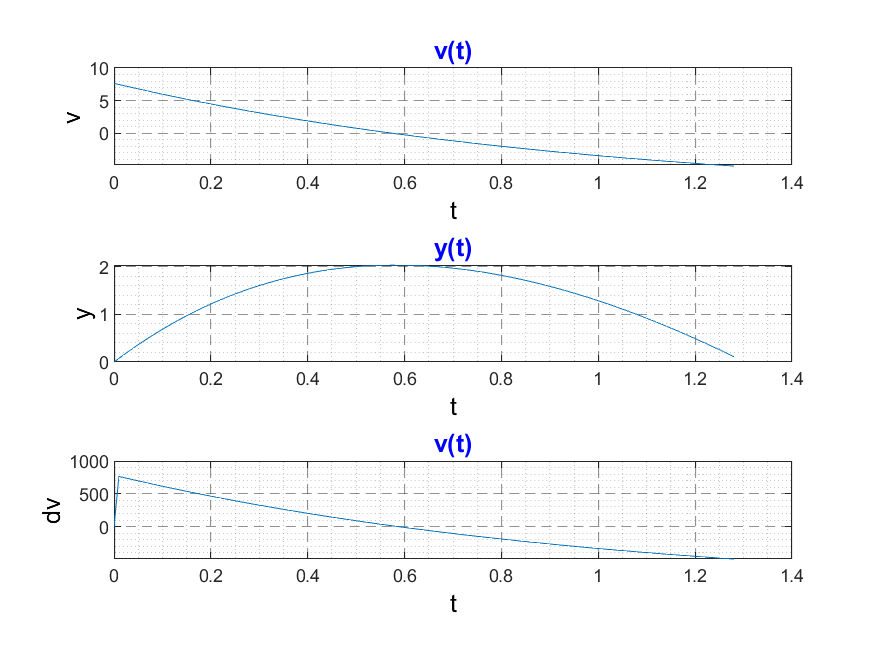
\includegraphics{cap/Elementary/img/script212}
    \GraphCap{Data-set}
    \label{fig:script212}
\end{figure}

